



%%%%%%%%%%%%%%%%%%%%%%%%%%%%%%%%%%%%%%%%%
% Beamer Presentation
% LaTeX Template
% Version 1.0 (10/11/12)
%
% This template has been downloaded from:
% http://www.LaTeXTemplates.com
%
% License:
% CC BY-NC-SA 3.0 (http://creativecommons.org/licenses/by-nc-sa/3.0/)
%
%%%%%%%%%%%%%%%%%%%%%%%%%%%%%%%%%%%%%%%%%

%----------------------------------------------------------------------------------------
%	PACKAGES AND THEMES
%----------------------------------------------------------------------------------------

\documentclass[aspectratio=169]{beamer}

\mode<presentation> {


% The Beamer class comes with a number of default slide themes
% which change the colors and layouts of slides. Below this is a list
% of all the themes, uncomment each in turn to see what they look like.

%\usetheme{default}
%\usetheme{AnnArbor}
%\usetheme{Antibes}
%\usetheme{Bergen}
%\usetheme{Berkeley}
%\usetheme{Berlin}
%\usetheme{Boadilla}
%\usetheme{CambridgeUS}
%\usetheme{Copenhagen}
%\usetheme{Darmstadt}
%\usetheme{Dresden}
%\usetheme{Frankfurt}
%\usetheme{Goettingen}
%\usetheme{Hannover}
%\usetheme{Ilmenau}
%\usetheme{JuanLesPins}
%\usetheme{Luebeck}
\usetheme{Madrid}
%\usetheme{Malmoe}
%\usetheme{Marburg}
%\usetheme{Montpellier}
%\usetheme{PaloAlto}
%\usetheme{Pittsburgh}
%\usetheme{Rochester}
%\usetheme{Singapore}
%\usetheme{Szeged}
%\usetheme{Warsaw}

% As well as themes, the Beamer class has a number of color themes
% for any slide theme. Uncomment each of these in turn to see how it
% changes the colors of your current slide theme.

%\usecolortheme{albatross}
%\usecolortheme{beaver}
%\usecolortheme{beetle}
%\usecolortheme{crane}
%\usecolortheme{dolphin}
%\usecolortheme{dove}
%\usecolortheme{fly}
%\usecolortheme{lily}
%\usecolortheme{orchid}
%\usecolortheme{rose}
%\usecolortheme{seagull}
%\usecolortheme{seahorse}
%\usecolortheme{whale}
%\usecolortheme{wolverine}

%\setbeamertemplate{footline} % To remove the footer line in all slides uncomment this line
%\setbeamertemplate{footline}[page number] % To replace the footer line in all slides with a simple slide count uncomment this line
\usepackage{amsmath}
\usepackage{selinput}      % Halbautomatische Auswahl der Eingabecodierung
\SelectInputMappings{      % mit Hilfe ausgewählter Glyphen
  adieresis={ä},	   % siehe: http://partners.adobe.com/public/developer/en/opentype/glyphlist.txt
  germandbls={ß},
  Euro={€}
}

\definecolor{UOSred}{rgb}{0.6745098039215686, 0.02352941176470588, 0.2039215686274510} % UBC Blue (primary)
\definecolor{UOSgrey}{rgb}{0.8117647058823529, 0.8117647058823529, 0.8117647058823529} % UBC Grey (secondary)

\setbeamercolor{palette primary}{bg=UOSred,fg=white}
\setbeamercolor{palette secondary}{bg=UOSred,fg=white}
\setbeamercolor{palette tertiary}{bg=UOSred,fg=white}
\setbeamercolor{palette quaternary}{bg=UOSred,fg=white}
\setbeamercolor{structure}{fg=UOSred} % itemize, enumerate, etc
\setbeamercolor{section in toc}{fg=UOSred} % TOC sections

%gets rid of bottom navigation bars
\setbeamertemplate{footline}[frame number]{}

%gets rid of bottom navigation symbols
\setbeamertemplate{navigation symbols}{}

\addtobeamertemplate{footline}{%
  \leavevmode%
  \hbox{%
  \begin{beamercolorbox}[wd=\paperwidth,ht=2.25ex,dp=1ex,center]{author in head/foot}%
     \insertsectionnavigationhorizontal{\paperwidth}{}{}
  \end{beamercolorbox}}%

}

% Override palette coloring with secondary
\setbeamercolor{subsection in head/foot}{bg=UOSgrey,fg=white}

%\setbeamertemplate{navigation symbols}{} % To remove the navigation symbols from the bottom of all slides uncomment this line
}
\usepackage{hyperref}
\usepackage{graphicx} % Allows including images
\usepackage{grffile}
\usepackage{booktabs} % Allows the use of \toprule, \midrule and \bottomrule in tables
\graphicspath{{images/}}
%----------------------------------------------------------------------------------------
%	TITLE PAGE
%----------------------------------------------------------------------------------------

\title[Aufgabe 1.1]{Aufgabe 1.1} % The short title appears at the bottom of every slide, the full title is only on the title page

\author{T. Adam, M. ben Ahmed} % Your name
\institute[UOS] % Your institution as it will appear on the bottom of every slide, may be shorthand to save space
{

Universität Osnabrück \\ % Your institution for the title page

\medskip
\textit{Algorithm Engineering} % Your email address


}
\date{\today} % Date, can be changed to a custom date

\begin{document}

\begin{frame}
\titlepage % Print the title page as the first slide
\end{frame}


%----------------------------------------------------------------------------------------
%	PRESENTATION SLIDES
%----------------------------------------------------------------------------------------


%------------------------------------------------

\begin{frame}
	\frametitle{Aufgabe 1.1 (a) - Externe Queue}
	\begin{columns}[c] % The "c" option specifies centered vertical alignment while the "t" option is used for top vertical alignment
	
	\column{.45\textwidth} % Left column and width
	\textbf{Queue}
	\begin{enumerate}
	\item \texttt{void enqueue(type v)}
	\item \texttt{type v dequeue()}
	\end{enumerate}
	
	\column{.5\textwidth} % Right column and width
	\begin{itemize}
		\item Queue funktioniert nach dem First-In/First-Out Prinzip (\textbf{FIFO})
		\item Array Implementation mit \textbf{front} und \textbf{rear} Zeiger
	\end{itemize}
	
	\end{columns}
	\end{frame}
%------------------------------------------------


\begin{frame}
	\frametitle{Aufgabe 1.1 (a) - Externe Queue}
	\begin{columns}[c] % The "c" option specifies centered vertical alignment while the "t" option is used for top vertical alignment
	
	\column{.45\textwidth} % Left column and width
	\textbf{Standard Queue}
	\begin{itemize}
		\item \emph{front}-Zeiger auf Anfang der Queue
		\item \emph{rear}-Zeiger auf Ende der Queue
		\item \texttt{enqueue()} an \emph{rear}
		\item \texttt{dequeue()} an \emph{front}
	\end{itemize}
	
	\column{.5\textwidth} % Right column and width
	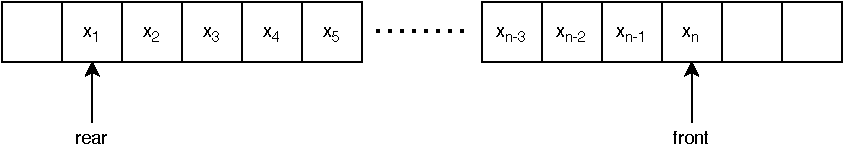
\includegraphics[scale=.5]{queue0.pdf}
	
	\end{columns}
	\end{frame}
%------------------------------------------------



\begin{frame}
	\frametitle{Aufgabe 1.1 (a) - Externe Queue}
	\begin{columns}[c] % The "c" option specifies centered vertical alignment while the "t" option is used for top vertical alignment
	
	\column{.45\textwidth} % Left column and width
	\textbf{Externe Queue}
	\begin{itemize}
		\item Falls $n>B$, halte nur ersten und letzten Block im Speicher
		\item Blöcke dazwischen $\rightarrow$ extern
	\end{itemize}
	
	\column{.5\textwidth} % Right column and width
	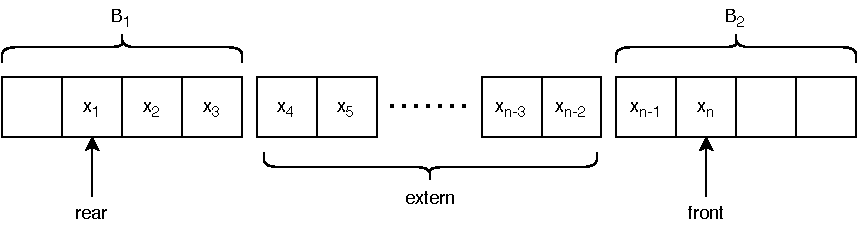
\includegraphics[scale=.5]{queue1.pdf}
	
	\end{columns}
	\end{frame}
%------------------------------------------------



\begin{frame}
	\frametitle{Aufgabe 1.1 (b) - Counting Sort}
	\begin{columns}[c] % The "c" option specifies centered vertical alignment while the "t" option is used for top vertical alignment
	
	\column{.45\textwidth} % Left column and width
	\begin{itemize}
		\item  array der Länge \emph{n}
		\item Elemente in \emph{i} müssen nicht eindeutig sein
		\item Temporäres array der Länge \emph{k}
		\item \emph{k} ist die Ziffer mit dem größten Wert
	\end{itemize}
	
	\column{.5\textwidth} % Right column and width
	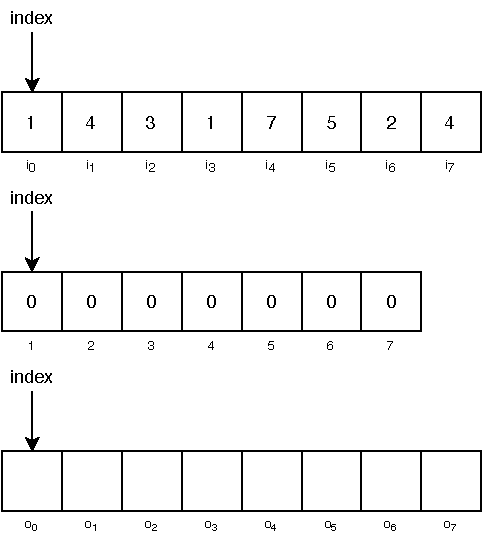
\includegraphics[scale=.7]{cs0.pdf}
	
	\end{columns}
	\end{frame}
%------------------------------------------------



\begin{frame}
	\frametitle{Aufgabe 1.1 (b) - Counting Sort}
	\begin{columns}[c] % The "c" option specifies centered vertical alignment while the "t" option is used for top vertical alignment
	
	\column{.45\textwidth} % Left column and width
	\begin{itemize}
		\item Input array wird durchlaufen
		\item Im temp. array wird gezählt wie oft jede Ziffer vorkommt
	\end{itemize}
	
	\column{.5\textwidth} % Right column and width
	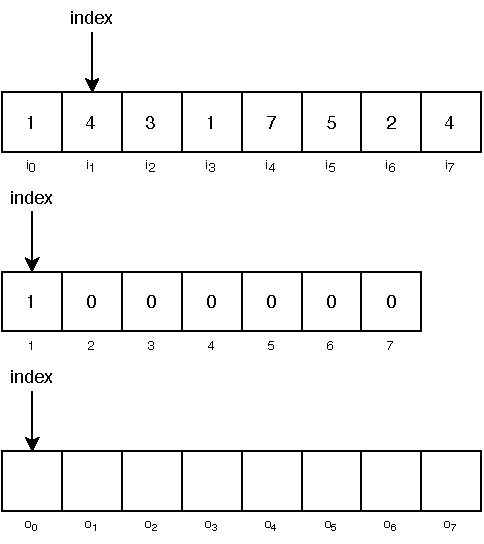
\includegraphics[scale=.7]{cs1.pdf}
	
	\end{columns}
	\end{frame}
%------------------------------------------------




\begin{frame}
	\frametitle{Aufgabe 1.1 (b) - Counting Sort}
	\begin{columns}[c] % The "c" option specifies centered vertical alignment while the "t" option is used for top vertical alignment
	
	\column{.45\textwidth} % Left column and width
	\begin{itemize}
		\item Input array wird durchlaufen
		\item Im temp. array wird gezählt wie oft jede Ziffer vorkommt
	\end{itemize}
	
	\column{.5\textwidth} % Right column and width
	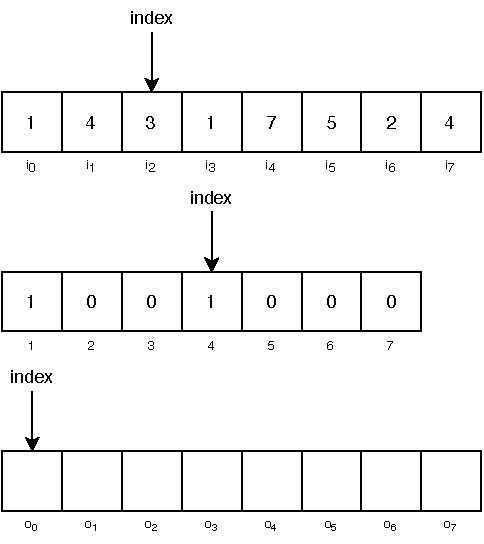
\includegraphics[scale=.7]{cs2.pdf}
	
	\end{columns}
	\end{frame}
%------------------------------------------------


\begin{frame}
	\frametitle{Aufgabe 1.1 (b) - Counting Sort}
	\begin{columns}[c] % The "c" option specifies centered vertical alignment while the "t" option is used for top vertical alignment
	
	\column{.45\textwidth} % Left column and width
	\begin{itemize}
		\item Input array wird durchlaufen
		\item Im temp. array wird gezählt wie oft jede Ziffer vorkommt
	\end{itemize}
	
	\column{.5\textwidth} % Right column and width
	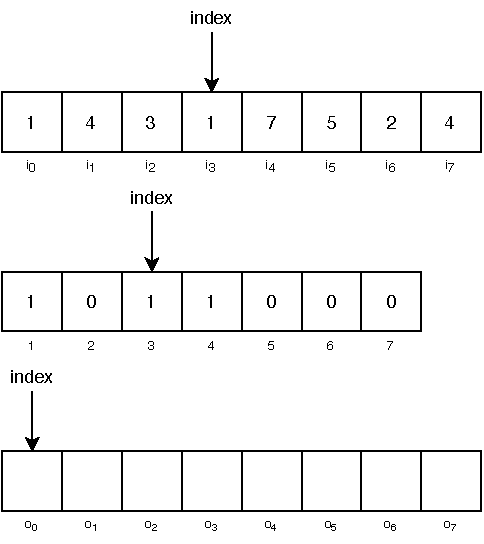
\includegraphics[scale=.7]{cs3.pdf}
	
	\end{columns}
	\end{frame}
%------------------------------------------------



\begin{frame}
	\frametitle{Aufgabe 1.1 (b) - Counting Sort}
	\begin{columns}[c] % The "c" option specifies centered vertical alignment while the "t" option is used for top vertical alignment
	
	\column{.45\textwidth} % Left column and width
	\begin{itemize}
		\item Input array wird durchlaufen
		\item Im temp. array wird gezählt wie oft jede Ziffer vorkommt
	\end{itemize}
	
	\column{.5\textwidth} % Right column and width
	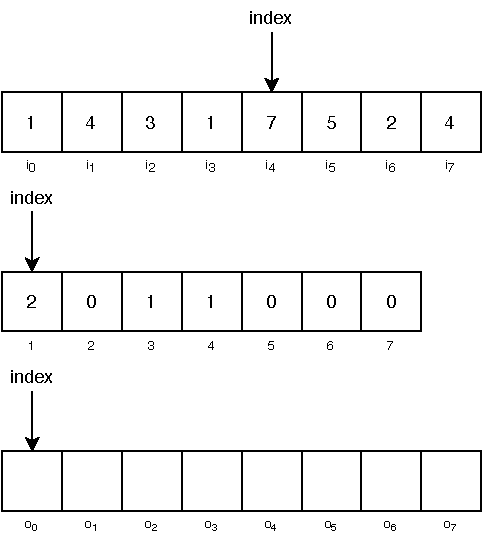
\includegraphics[scale=.7]{cs4.pdf}
	
	\end{columns}
	\end{frame}
%------------------------------------------------




\begin{frame}
	\frametitle{Aufgabe 1.1 (b) - Counting Sort}
	\begin{columns}[c] % The "c" option specifies centered vertical alignment while the "t" option is used for top vertical alignment
	
	\column{.45\textwidth} % Left column and width
	\begin{itemize}
		\item Das temp. array enthält die Anzahl der gleichen Elemente
	\end{itemize}
	
	\column{.5\textwidth} % Right column and width
	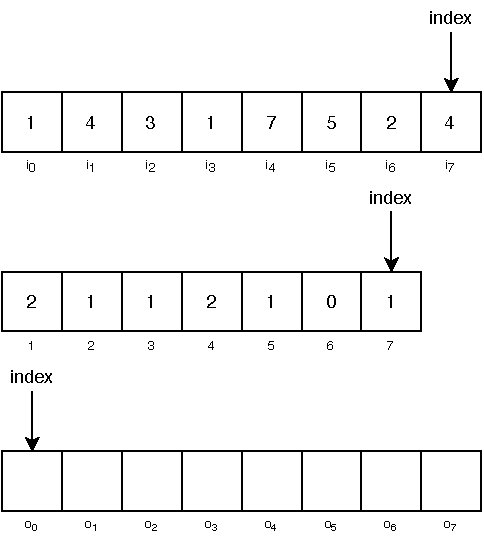
\includegraphics[scale=.7]{cs5.pdf}
	
	\end{columns}
	\end{frame}
%------------------------------------------------



\begin{frame}
	\frametitle{Aufgabe 1.1 (b) - Counting Sort}
	\begin{columns}[c] % The "c" option specifies centered vertical alignment while the "t" option is used for top vertical alignment
	
	\column{.45\textwidth} % Left column and width
	\begin{itemize}
		\item Einträge des temp. array werden paarweise addiert
		\item Summe wird in die jeweils rechte Zelle eingetragen
	\end{itemize}
	
	\column{.5\textwidth} % Right column and width
	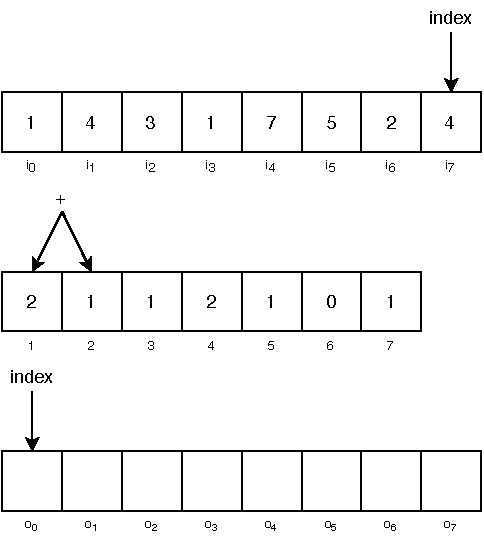
\includegraphics[scale=.7]{cs6.pdf}
	
	\end{columns}
	\end{frame}
%------------------------------------------------


\begin{frame}
	\frametitle{Aufgabe 1.1 (b) - Counting Sort}
	\begin{columns}[c] % The "c" option specifies centered vertical alignment while the "t" option is used for top vertical alignment
	
	\column{.45\textwidth} % Left column and width
	\begin{itemize}
		\item Einträge des temp. array werden paarweise addiert
		\item Summe wird in die jeweils rechte Zelle eingetragen
	\end{itemize}
	
	\column{.5\textwidth} % Right column and width
	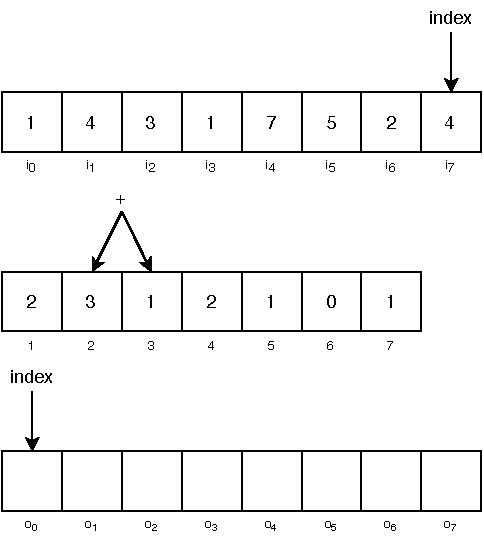
\includegraphics[scale=.7]{cs7.pdf}
	
	\end{columns}
	\end{frame}
%------------------------------------------------


\begin{frame}
	\frametitle{Aufgabe 1.1 (b) - Counting Sort}
	\begin{columns}[c] % The "c" option specifies centered vertical alignment while the "t" option is used for top vertical alignment
	
	\column{.45\textwidth} % Left column and width
	\begin{itemize}
		\item Einträge des temp. array werden paarweise addiert
		\item Summe wird in die jeweils rechte Zelle eingetragen
	\end{itemize}
	
	\column{.5\textwidth} % Right column and width
	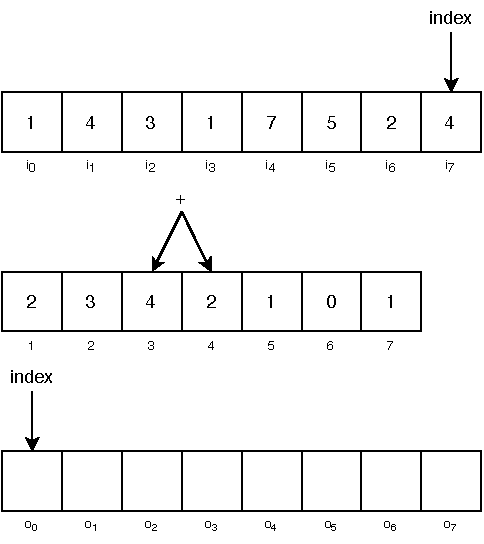
\includegraphics[scale=.7]{cs8.pdf}
	
	\end{columns}
	\end{frame}
%------------------------------------------------



\begin{frame}
	\frametitle{Aufgabe 1.1 (b) - Counting Sort}
	\begin{columns}[c] % The "c" option specifies centered vertical alignment while the "t" option is used for top vertical alignment
	
	\column{.45\textwidth} % Left column and width
	\begin{itemize}
		\item Alle Einträge wurden aufsummiert
		\item Es ergibt sich eine aufsteigende Reihenfolge
	\end{itemize}
	
	\column{.5\textwidth} % Right column and width
	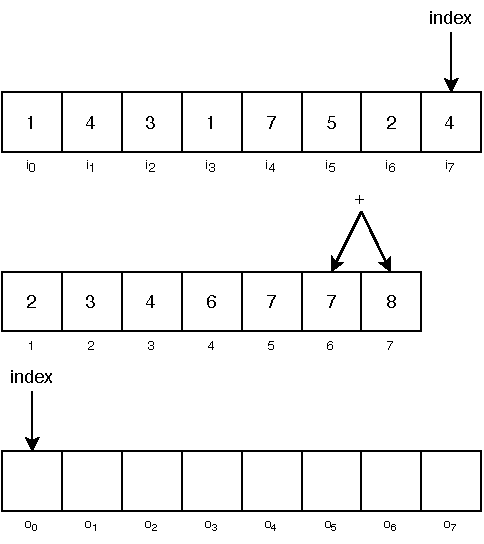
\includegraphics[scale=.7]{cs9.pdf}
	
	\end{columns}
	\end{frame}
%------------------------------------------------


\begin{frame}
	\frametitle{Aufgabe 1.1 (b) - Counting Sort}
	\begin{columns}[c] % The "c" option specifies centered vertical alignment while the "t" option is used for top vertical alignment
	
	\column{.45\textwidth} % Left column and width
	\begin{itemize}
		\item Input array wird rückwärts durchlaufen
		\item Es wird an der i-ten Stelle des temp. arrays nach dem output Index geschaut
	\end{itemize}
	
	\column{.5\textwidth} % Right column and width
	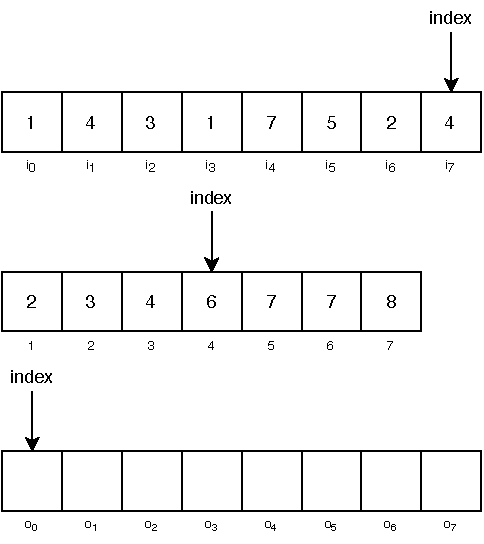
\includegraphics[scale=.7]{cs10.pdf}
	
	\end{columns}
	\end{frame}
%------------------------------------------------


\begin{frame}
	\frametitle{Aufgabe 1.1 (b) - Counting Sort}
	\begin{columns}[c] % The "c" option specifies centered vertical alignment while the "t" option is used for top vertical alignment
	
	\column{.45\textwidth} % Left column and width
	\begin{itemize}
		\item Element aus dem input array wird an die entsprechende Stelle im output array geschrieben
	\end{itemize}
	
	\column{.5\textwidth} % Right column and width
	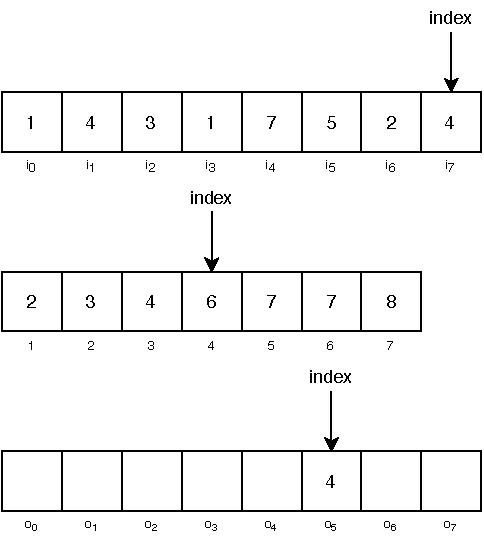
\includegraphics[scale=.7]{cs11.pdf}
	
	\end{columns}
	\end{frame}
%------------------------------------------------

\begin{frame}
	\frametitle{Aufgabe 1.1 (b) - Counting Sort}
	\begin{columns}[c] % The "c" option specifies centered vertical alignment while the "t" option is used for top vertical alignment
	
	\column{.45\textwidth} % Left column and width
	\begin{itemize}
		\item Wert im temp. array wird um 1 dekrementiert
	\end{itemize}
	
	\column{.5\textwidth} % Right column and width
	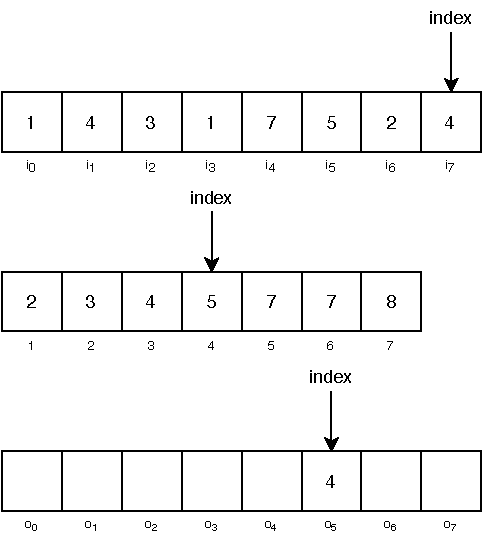
\includegraphics[scale=.7]{cs12.pdf}
	
	\end{columns}
	\end{frame}
%------------------------------------------------


\begin{frame}
	\frametitle{Aufgabe 1.1 (b) - Counting Sort}
	\begin{columns}[c] % The "c" option specifies centered vertical alignment while the "t" option is used for top vertical alignment
	
	\column{.45\textwidth} % Left column and width
	\begin{itemize}
		\item Element aus dem input array wird an die entsprechende Stelle im output array geschrieben
	\end{itemize}
	
	\column{.5\textwidth} % Right column and width
	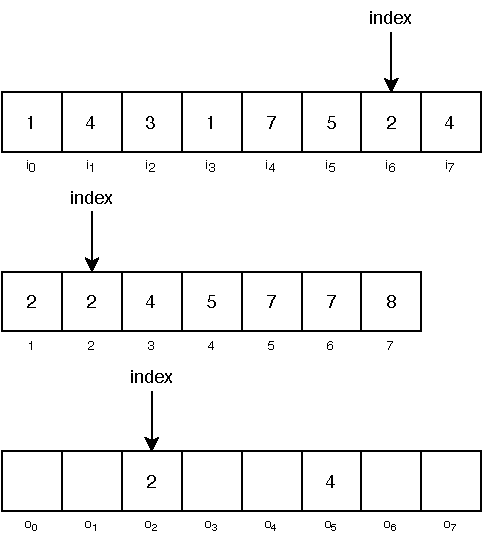
\includegraphics[scale=.7]{cs13.pdf}
	
	\end{columns}
	\end{frame}
%------------------------------------------------


\begin{frame}
	\frametitle{Aufgabe 1.1 (b) - Counting Sort}
	\begin{columns}[c] % The "c" option specifies centered vertical alignment while the "t" option is used for top vertical alignment
	
	\column{.45\textwidth} % Left column and width
	\begin{itemize}
		\item Im output array befinden sich die sortierten Werte des input arrays
		\item Insbesondere bleibt die Reihenfolge gleicher Elemente erhalten
	\end{itemize}
	
	\column{.5\textwidth} % Right column and width
	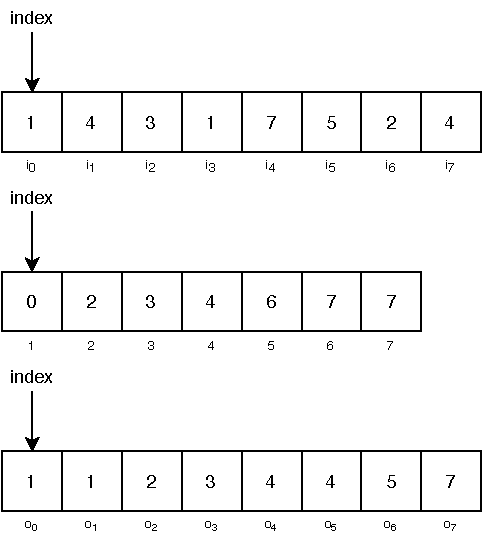
\includegraphics[scale=.7]{cs14.pdf}
	
	\end{columns}
	\end{frame}
%------------------------------------------------


\begin{frame}
	\frametitle{Aufgabe 1.1 (b) - Counting Sort}
	\begin{columns}[c] % The "c" option specifies centered vertical alignment while the "t" option is used for top vertical alignment
	
	\column{.45\textwidth} % Left column and width
	\textbf{I/O Fallunterscheidung}
	\begin{enumerate}
	\item $ k = \alpha \cdot M $ mit $\alpha = 0,5$
	\item $ k = \alpha \cdot M $ mit $\alpha > 1$ \pause
	\end{enumerate}
	

	\column{.5\textwidth} % Right column and width
	\begin{itemize}
		\item Temp. array passt vollständig in den Speicher $\rightarrow$ keine I/O \pause
		\item Temp. array passt nicht in den Speicher $\rightarrow$ viele I/O
	\end{itemize}
	
	\end{columns}
	\end{frame}
%------------------------------------------------


\end{document} 